\section{Развитие проекта EXPERTroot. Методы обработки данных.}
\label{section:processing}

%\red{, соответствует своему, ожидаемому, интервалу возможных значений величины $\delta \tau$, см. формулу \ref{koordinate}.}
%\red{Сравнивая ожидаемое $\Delta \tau$, с экспериментально полученным распределением, можно оценить насколько точно мы можем определять пространственное положение взаимодействия налетающей частицы с материалом детектора. Tо есть пространственное разрешение детектора, а дисперсия распределения величины $\delta \tau$ характеризует временное разрешение.}


Для обработки данных также использовался программный пакет \er.
Функции разработанные в рамках представленной работы были применены для обработки данных детектора NeuRad, но благодаря своей универсальности могут быть применены и для других детекторов.

В качестве развития проекта \er, в существующий фреймворк были внедрены методы для считывания и обработки набранных данных. С помощью разработанных алгоритмов можно анализировать любые амплитудные и временные характеристики оцифрованных импульсов, записанных в файлах любого формата: текстовых, бинарных и других. В фреймворк были внедрены известные методы дискриминации и анализа формы сигнала, такие как дискриминатор переднего фронта (Leading-Edge Discriminator), дискриминатор со следящим порогом (Constant-Fraction Discriminator), расчёт времени сигнала над порогом (Time-over-Threshold), поиск максимума амплитуды, расчёт среднего уровня шума, расчёт интегральной суммы амплитуд и другие. Хотя вышеперечисленные методы обычно существуют в обычном осциллографе, преимуществом использования разработанных алгоритмов на базе существующего фреймворка является то, что в неё в любой момент можно с лёгкостью добавить новые методы анализа сигналов. Таким образом, функциональность \er\ относительно обработки сигналов огромна по сравнению с ограниченным списком методов анализа любого считывающего устройства. 

%Используя существующие библиотеки, нам удалось внедрить в неё известные методы обработки данных, такие как метод дискриминатор переднего фронта (Leading-Edge Discriminator), дискриминатор со следящим порогом (Constant-Fraction Discriminator) и другие.
%Ниже описаны внедрённые алгоритмы анализа формы импульса сигналов и параметры, расчёт которых производит программа.

При анализе сигналов все амплитудные характеристики сигналов были рассчитаны относительно оцененного среднего уровня шума. Последний рассчитывался для каждого канала фитированием шумовой части сигнала каждого события функцией $y=A$, где А - параметр прямой горизонтальной линии. Поэтому, на Рис.\ref{ris:signal1} уровень шумовой дорожки в среднем находится в $U$=0\,V.

%Исходя из того, что исходные сохранённые сигналы представляют собой дискретный набор амплитуд и времён, то более точно момент превышения порога сигналом лучше определять, как временную координату точки пересечения непрерывного \red{графа}, полученного из оцифрованных, дискретных значений амплитуд и времён с помощью линейной аппроксимации соседних по времени значений, с горизонтальной линией порога.  

Исходя из того, что исходные сохранённые сигналы представляют собой дискретный набор амплитуд и времён, то для более точного анализа характеристик сигналов были использованы объекты класса TGraph и дальнейшие методы обработки использовались на интерполированных значениях записанных точек.

Рассмотрим один из основных внедрённых в программу методов: \textbf{дискриминатор переднего фронта} - Leading Edge Discriminator (LED) \cite{methods}.  Установив определённый порог (Рис.~\ref{ris:LED}), можно получить время превышения порога передним фронтом сигнала (time mark) и длительность превышения сигналом данного порога (Time-over-Threshold), так называемое время сигнала над порогом. %Временем прихода сигнала, в данном методе является - момент отмеченный на рис.\ref{ris:LED} как "time mark".
Временем прихода сигнала можно считать момент превышения сигналом выбранного порога. 

\begin{figure}[!h]
	\center{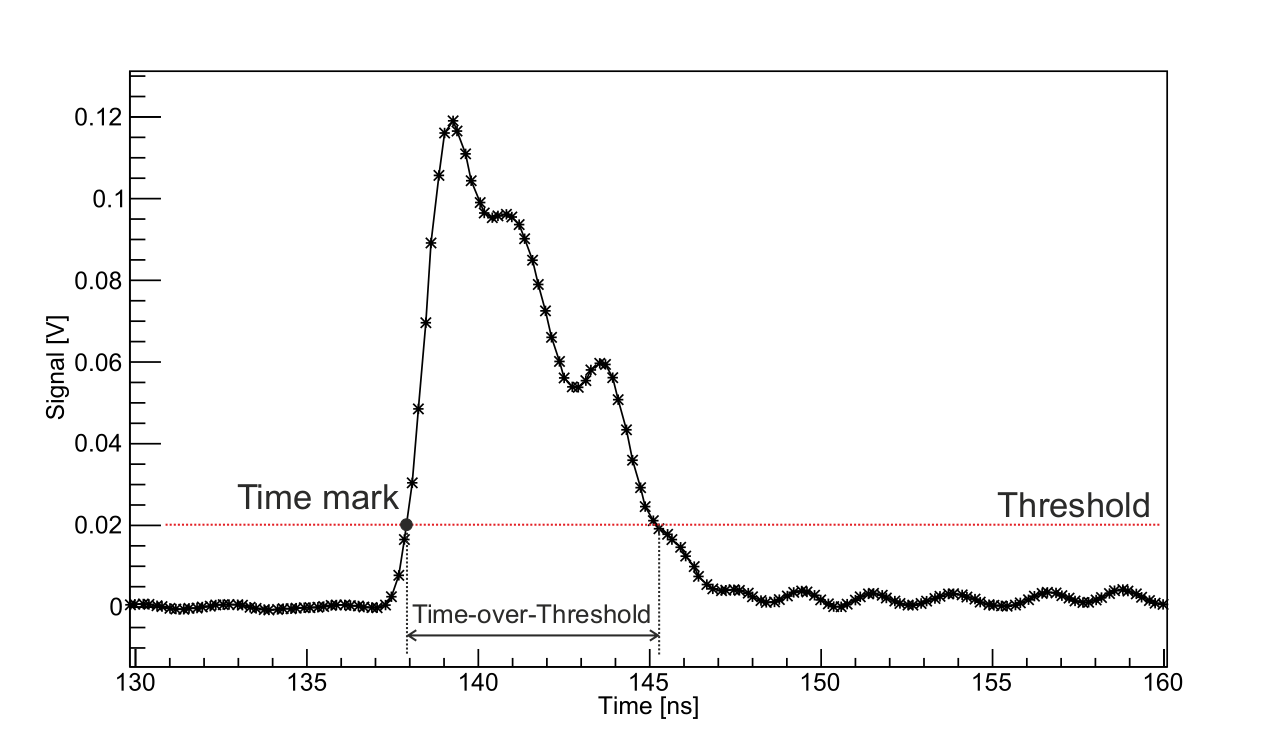
\includegraphics[width=1\linewidth]{LED1.png}}
	\caption{Анализ переднего фронта. Time mark - время сигнала, определяется как пересечение линии фитирования фронта и нулевого уровня.}
	\label{ris:LED}
\end{figure}
%{
%	\centering
%	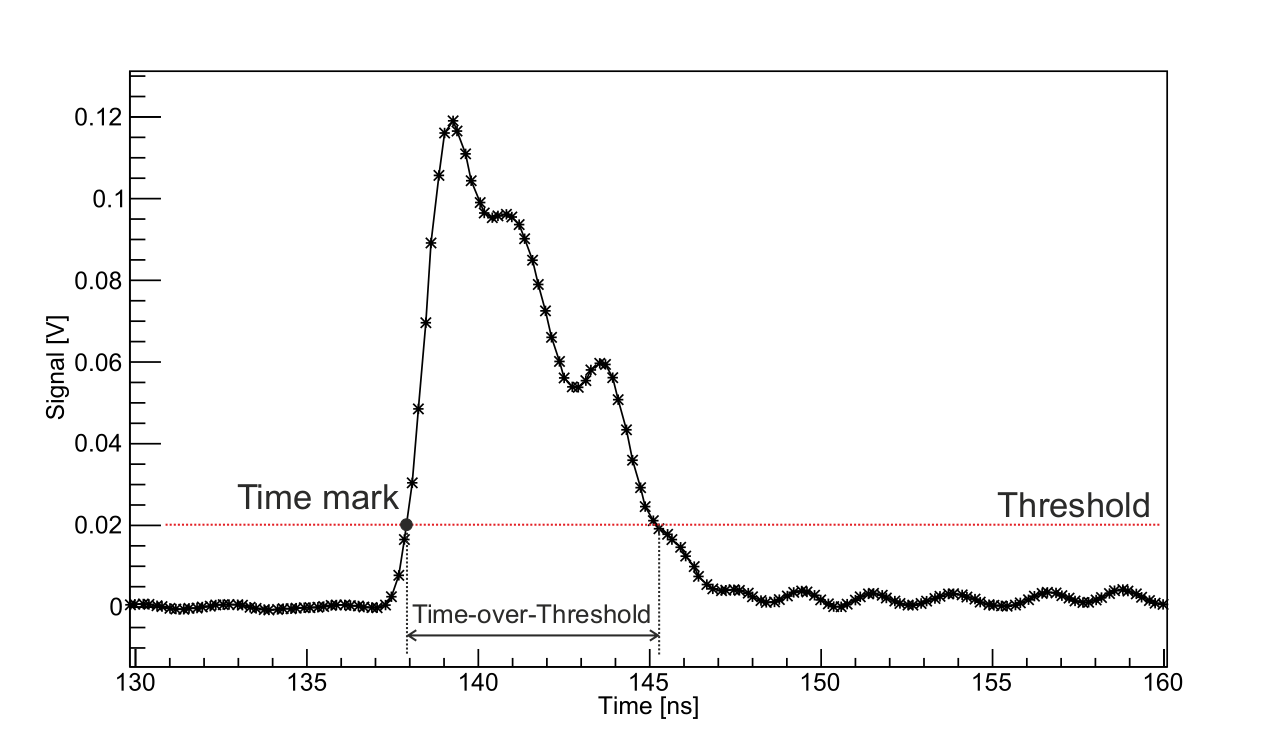
\includegraphics[width=1\linewidth]{LED1.png}
%	\captionof{figure}{Анализ переднего фронта. Time mark - время прихода сигнала, определяется пересечением непрерывного графа и установленного уровня.}\label{ris:LED}
%}

Следующий метод определения времени сигнала основан на анализе переднего фронта сигнала. \textbf{Передний фронт} определялся как область нарастающей части сигнала, ограниченная первым локальным максимом сигнала и началом нарастания сигнала. Первый локальный максимум определяется, как точка первого перегиба формы сигнала от нарастания к убыванию, при условии, что амплитуда в этой точке превышает выбранный порог. Последнее условие необходимо для отсеивания локальных максимумов, возникающих на уровне шумов. Для сигналов, полученных в проведённых экспериментах значение порога было равно 20\,mV. 
Время прихода сигнала рассматривали как время достижения 10, 50 или 90\% от значения амплитуды первого локального максимума.

Следующий способ получить время сигнала: \textbf{дискриминатор со следящим порогом} - Constant Fraction Discriminator (CFD)~\cite{methods}. Идея этого метода состоит в том, что временная привязка определяется не постоянным порогом, а моментом, когда входной импульс достигает определенной доли (например, половины) амплитудного значения. Очевидно, что для импульсов одинаковой формы этот момент не зависит от амплитуды.
Реализация метода иллюстрируется на рис.~\ref{ris:cfd}.
Входной сигнал разветвляется на два канала. В одном из каналов сигнал задерживается на величину, несколько меньшую длины переднего фронта импульса. В другом канале сигнал ослабляется и инвертируется. Затем оба сигнала суммируются, и в результате получается биполярный импульс, причем время пересечения нуля зависит от двух параметров (времени задержки и коэффициента ослабления) и не зависит от амплитуды для сигналов одинаковой формы. Параметры схемы подбираются экспериментально, исходя из целей получения наилучшего временного разрешения и наиболее полной компенсации амплитудной зависимости.

\begin{figure}[!t]
	\center{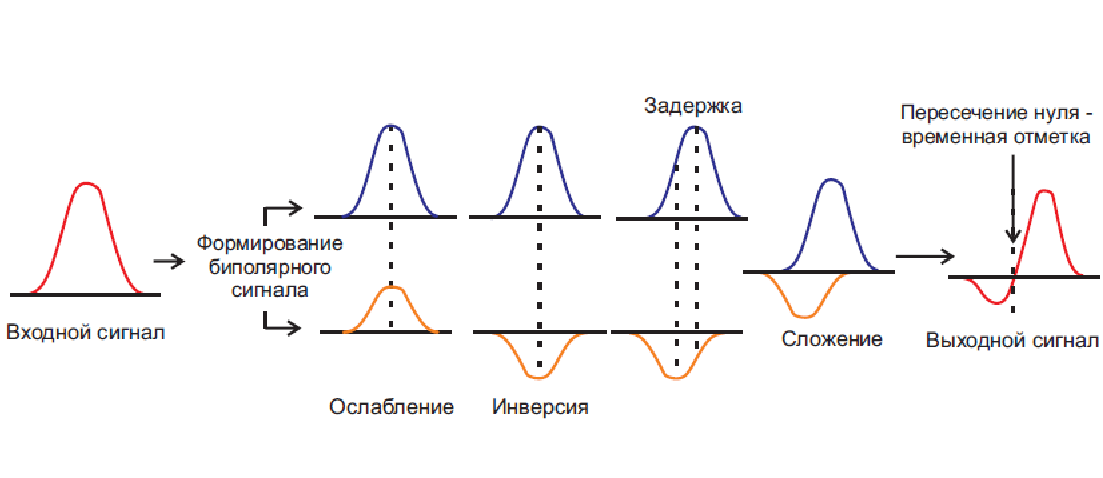
\includegraphics[width=1\linewidth]{cfd.png}}
	\caption{ Схематическая иллюстрация аппаратного метода устранения амплитудно-временной зависимости временной отметки – метод Constant Fraction Discriminator (CFD).  Красным цветом показаны формы входного и выходного (биполярный импульс) сигналов. Синим и оранжевым цветом показаны формы сигналом на этапах обработки: формирование биполярного сигнала из входного, ослабление и инверсия одного из сформированных сигналов,  задержка по времени другого, и результирующее суммирование.}
	\label{ris:cfd}
\end{figure}

Для иллюстрации, исходный сигнал записанный оцифровывающим устройством показан на Рис.~\ref{ris:CFDform}a), а преобразованный выходной на Рис.~\ref{ris:CFDform}b).
В данном случае параметр ослабления был равен 0.3, то есть: инвертированный сигнал ослаблялся на 70\%, и задерживался на 1.5\,нс.
Метод CFD лучше всего работает для сигналов с постоянной формой импульса. Для таких сигналов, сравнивая точность временных отметок, полученных с дискриминатора переднего фронта и с дискриминатора со следящим порогом, во втором случае неопределенность временной отметки несколько больше. Это связано с тем, что при сложении двух сигналов в методе CFD происходит небольшое уменьшение крутизны фронта сигнала \cite{dasha}.

\begin{figure}[!h]
	\centering
	\begin{tabular}{cc}
		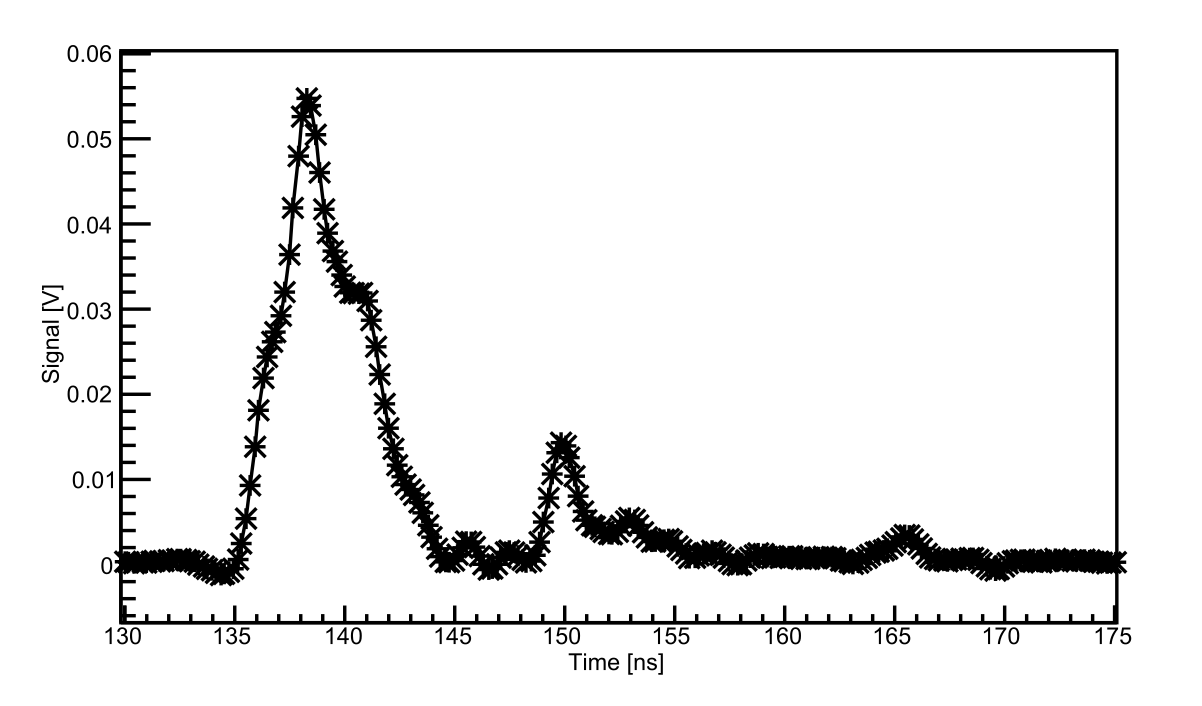
\includegraphics[width=0.5\linewidth]{originalsignalform.png} & 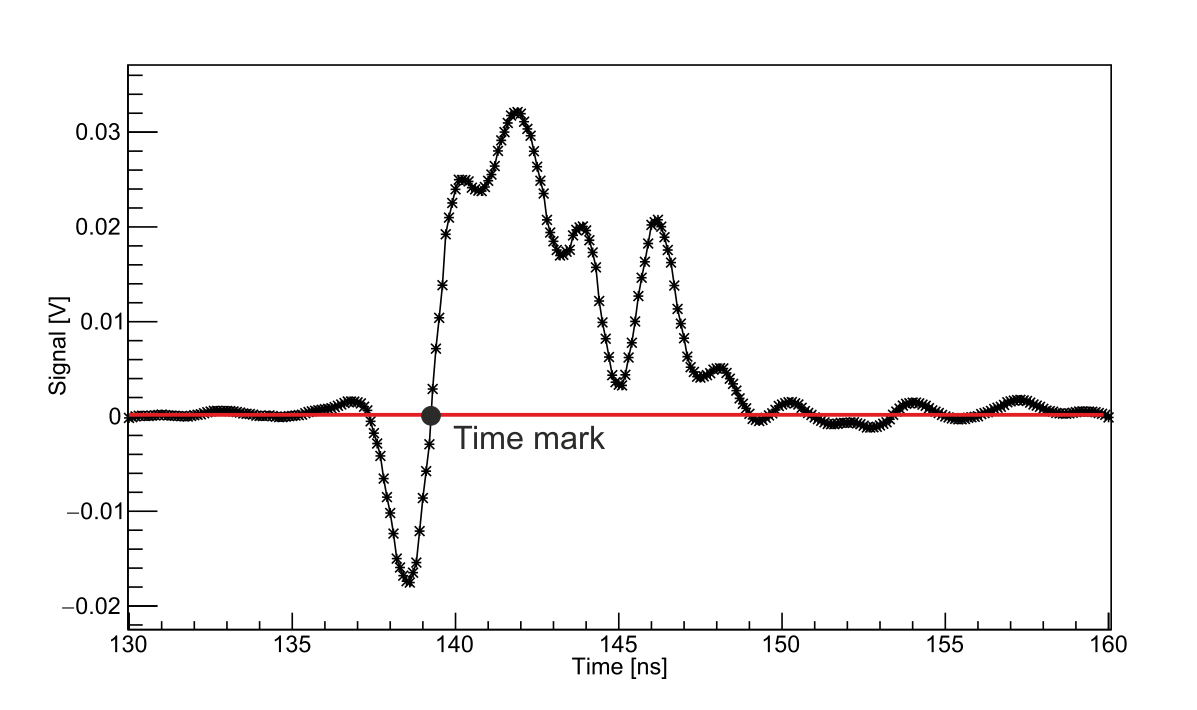
\includegraphics[width=0.5\linewidth]{CFDform.png} \\
		a) & b) \\
	\end{tabular}
	\caption{a) Исходный сигнал полученный в измерении с прототипом NeuRad, описанной в главе\,\ref{sec:timeTests}. b) Выходной, преобразованный сигнал методом следящего порога с коэффициентом ослабления 0.3 и задержкой 1.5 нс.}\label{ris:CFDform}
\end{figure}

Обобщая вышеизложенное, можно заключить, что для проведения качественных прецизионных измерений времени необходимы входные сигналы с высоким значением крутизны фронта и незначительными шумами.

%\begin{figure}[h]
%	\center{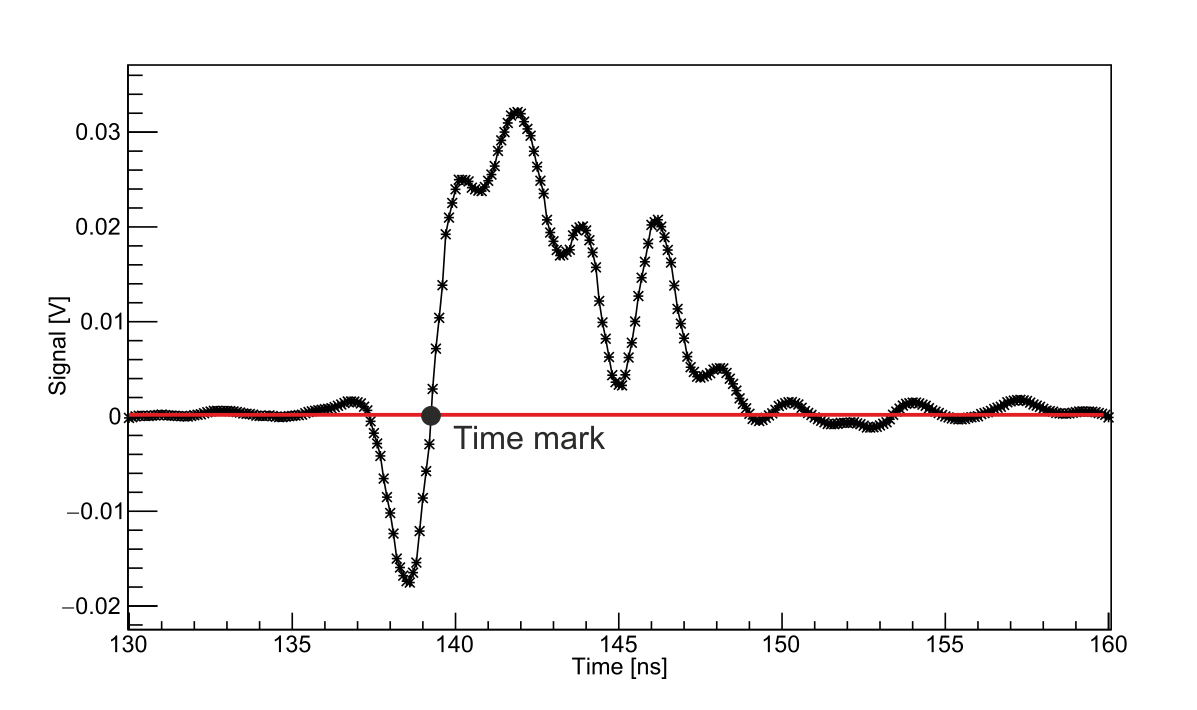
\includegraphics[width=1\linewidth]{CFDform.png}}
%	\caption{Выходной, преобразованный сигнал методом следящего порога с коэффициентом ослабления 0.3 и задержкой 1.5 нс.}
%	\label{ris:CFDform}
%\end{figure}
%{
%	\centering
%	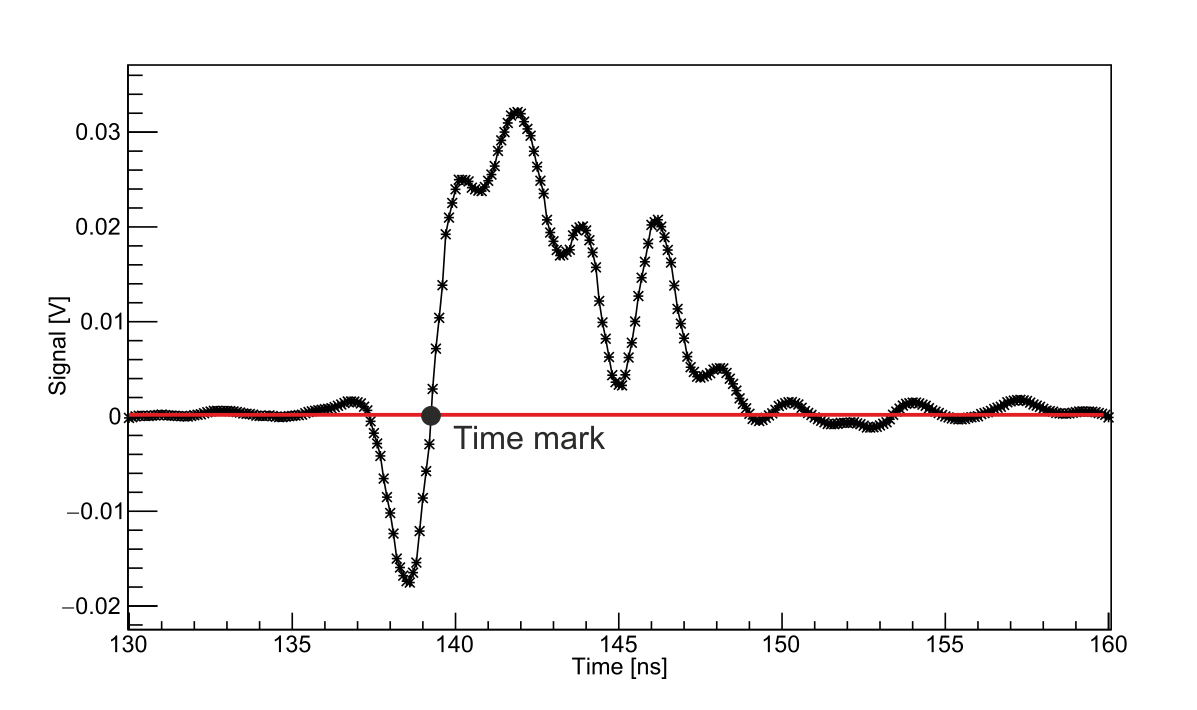
\includegraphics[width=1\linewidth]{CFDform.png}
%	\captionof{figure}{Выходной, преобразованный сигнал методом следящего порога с коэффициентом ослабления 0.3 и задержкой 1.5 нс.}\label{ris:CFDform}
%}


Один из важных рассчитывающийся параметров - это \textbf{время сигнала над порогом}, или, так называемое "Time-over-Threshold (ToT)"\ (см. Рис.~\ref{ris:LED}). Время сигнала над порогом является важным параметром для отбора сигналов в зависимости от поставленной физической задачи.
Очевидно, что в нашем эксперименте из всех записанных сигналов представляли интерес только сигналы с большим значением ToT. Например, сигналы, возникающие при спонтанной эмиссии одного или нескольких электронов с фотокатода ФЭУ такими не являются и могут быть отсеяны отбором по параметру ToT. Сигналы с таким эффектом можно наблюдать достаточно часто и, как правило, сигнал от таких событий виден только на одном из двух ФЭУ.
Для иллюстрации на Рис.~\ref{ris:noise} показаны два сигнала из одного события. На верхней панели показан сигнал зарегистрированный по триггеру, источником которого является одноэлектронная эмиссия, причем на втором ФЭУ в том же событии видим только шумовую дорожку.

\begin{figure}[!h]
	\center{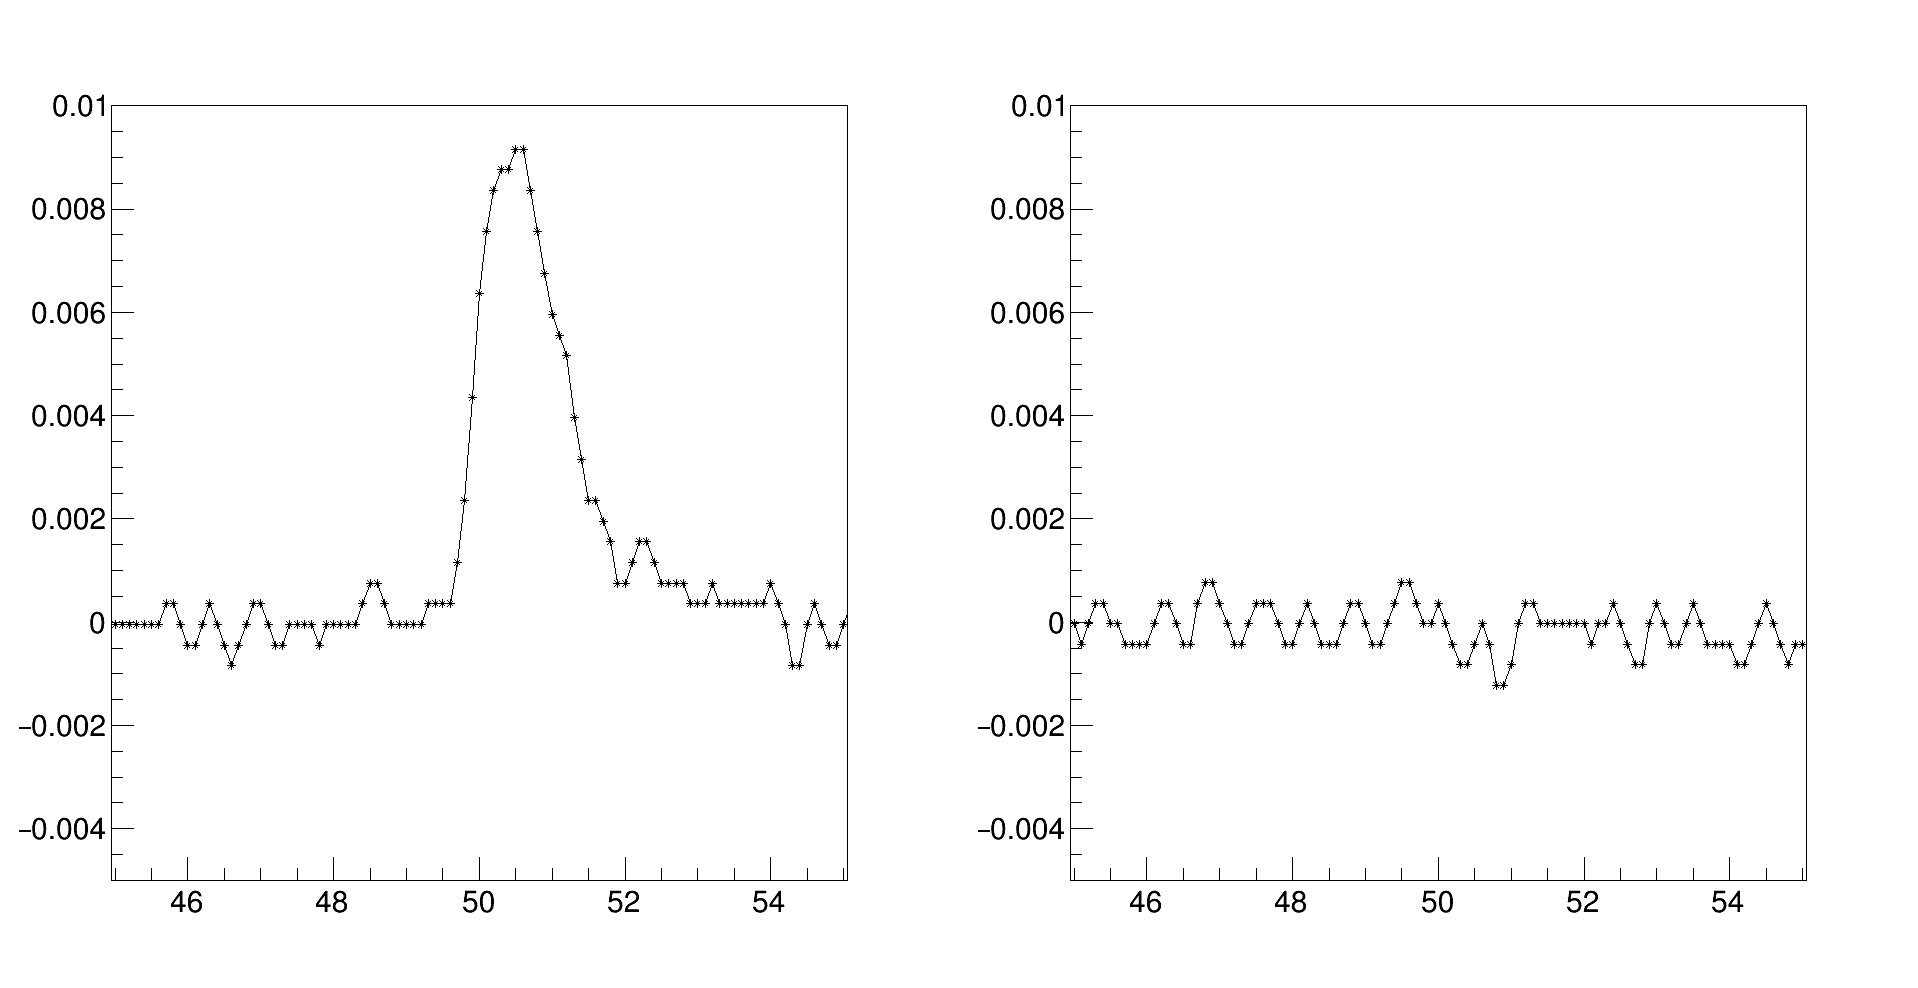
\includegraphics[width=1\linewidth]{noise.png}}
	\caption{Сигналы с обоих концов прототипа NeuRad при отсутствии источника. Одноэлектронный шум присутствует в канале только с одной стрроны.}
	\label{ris:noise}
\end{figure}

Полезным параметром для отбора необходимых сигналов является заряд, зарегистрированный анодом
\begin{equation}
%Q = \frac{1}{R}\, \int_{\tau_1}^{\tau_2} U(t)\, dt,
Q = \frac{1}{R}\, \int\limits^{\tau_1}_{\tau_2} U(t)\, dt,
\label{charge}
\end{equation}
где $U(t)$ -- амплитуда сигнала в момент времени $t$, $\tau_1$ и $\tau_2$ -- время начала и окончания сигнала соответственно, $R$-постоянное сопротивление устройства (50\,Ом) \cite{vratislav}. Оценивая суммарную форму сигнала можно определить среднее время нарастания фронта сигнала и характерное время его спада. 
Для проведённых экспериментов были проведены оценки: $\tau_1 = \tau_{max} - 3\,$нс и $\tau_2 = \tau_{max} + 17\,$нс, где $\tau_{max}$ - время максимальной амплитуды сигнала. То есть, интегральная сумма формы сигнала рассчитывалась в 20 наносекундном окне, начиная с момента 3\,нс до достижения максимума.

Для оценки правдоподобности методов обработки оценивалось время высвечивания сцинтиллятора.
%Наиболее простое приближение зависимости интенсивности высвечивания от времени органического сцинтиллятора имеет вид .
Пользуясь законом \eqref{scintSHAPE}, и зная среднюю, либо суммарную форму сигнала, можно оценить параметр высвечивания, фитированием заднего фронта сигнала убывающей экспоненциальной функцией.

%\begin{figure}[!h]
%	\center{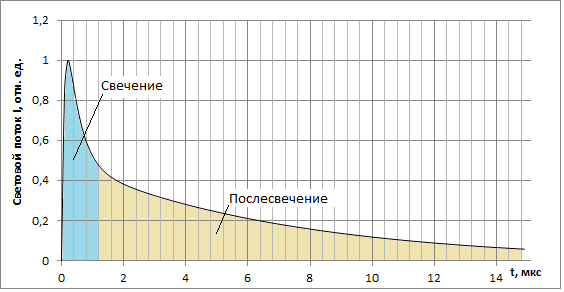
\includegraphics[width=1\linewidth]{scintSHAPE.png}}
%	\caption{Типичная кривая высвечивания неорганического сцинтиллятора, возбуждённого поглощением быстрой заряженной частицы. После кратковременной яркой вспышки свечение относительно медленно затухает.}
%	\label{ris:scintSHAPE}
%\end{figure}

Другой немаловажный параметр, с помощью которого можно проверить качество измерений - время нарастания сигнала, определяющийся, как время, за которое амплитуда сигнала увеличивается с 10 до 90 процентов амплитуды максимума переднего фронта сигнала. Так как, записанные сигналы отличаются по форме, то время нарастания можно оценивать также по суммарной форме сигнала. Причиной не мгновенного нарастания сигнала является наличие временного разрешения ФЭУ, так как основная часть светового сигнала достигает фотокатода практически мгновенно. 
%Для оценки качества результатов обработки, было проведено сравнение полученного времени нарастания переднего фронта с временным разрешением ФЭУ.
